\section{Evaluation}
\label{sec:evaluation}

We evaluated three policy variants via trace-driven co-simulation. RC parameters are validated from the gem5 full-system smoke run (\texttt{config.ini}, Workstream~A). Power and IPC baselines are gem5-calibrated: big cluster $P_{dyn}$\,=\,2.21\,W, IPC\,=\,0.991 at 3.3\,GHz; LITTLE cluster $P_{dyn}$\,=\,0.86\,W, IPC\,=\,0.653 at 2.0\,GHz (from \texttt{stats.txt}, 113 dumps). All results are \emph{modeled}, not measured on hardware.

\subsection{Simulation Setup}

The co-simulation architecture mirrors a modern ARM big.LITTLE SoC:
\begin{itemize}
    \item \textbf{big Cluster:} OPP peak \SI{4.5}{\watt} at 3.3\,GHz (theoretical TDP); gem5-simulated mean \SI{2.21}{\watt}.
    \item \textbf{LITTLE Cluster:} \SI{0.86}{\watt} mean at 2.0\,GHz (gem5-calibrated).
    \item \textbf{Thermal Constraints:} $T_{proact} = \SI{75}{\degreeCelsius}$, $T_{throttle} = \SI{85}{\degreeCelsius}$, $T_{amb} = \SI{25}{\degreeCelsius}$.
    \item \textbf{RC Parameters (gem5-validated):} $R_1\!=\!5$, $R_2\!=\!2$, $R_3\!=\!8$\,K/W; $C_1\!=\!1$, $C_2\!=\!5$, $C_3\!=\!15$\,J/K; $\tau_{hs}\!=\!120$\,s.
\end{itemize}

Three variants are compared over 600 simulated seconds under a sustained peak-OPP load:
\begin{enumerate}
    \item \textbf{V1 — 2-node + aggressive DVFS:} Legacy baseline; uses 2-node RC and steps down frequency at $T_{die} \geq T_{proact}$.
    \item \textbf{V2 — 3-node + balanced DVFS:} Improved thermal model; same DVFS policy.
    \item \textbf{V3 — 3-node + Phase~6 policy:} Package-aware; defers DVFS via migration when $T_{pkg} < 65\,\text{°C}$.
\end{enumerate}

\subsection{Results}

\begin{figure}[t]
\centering
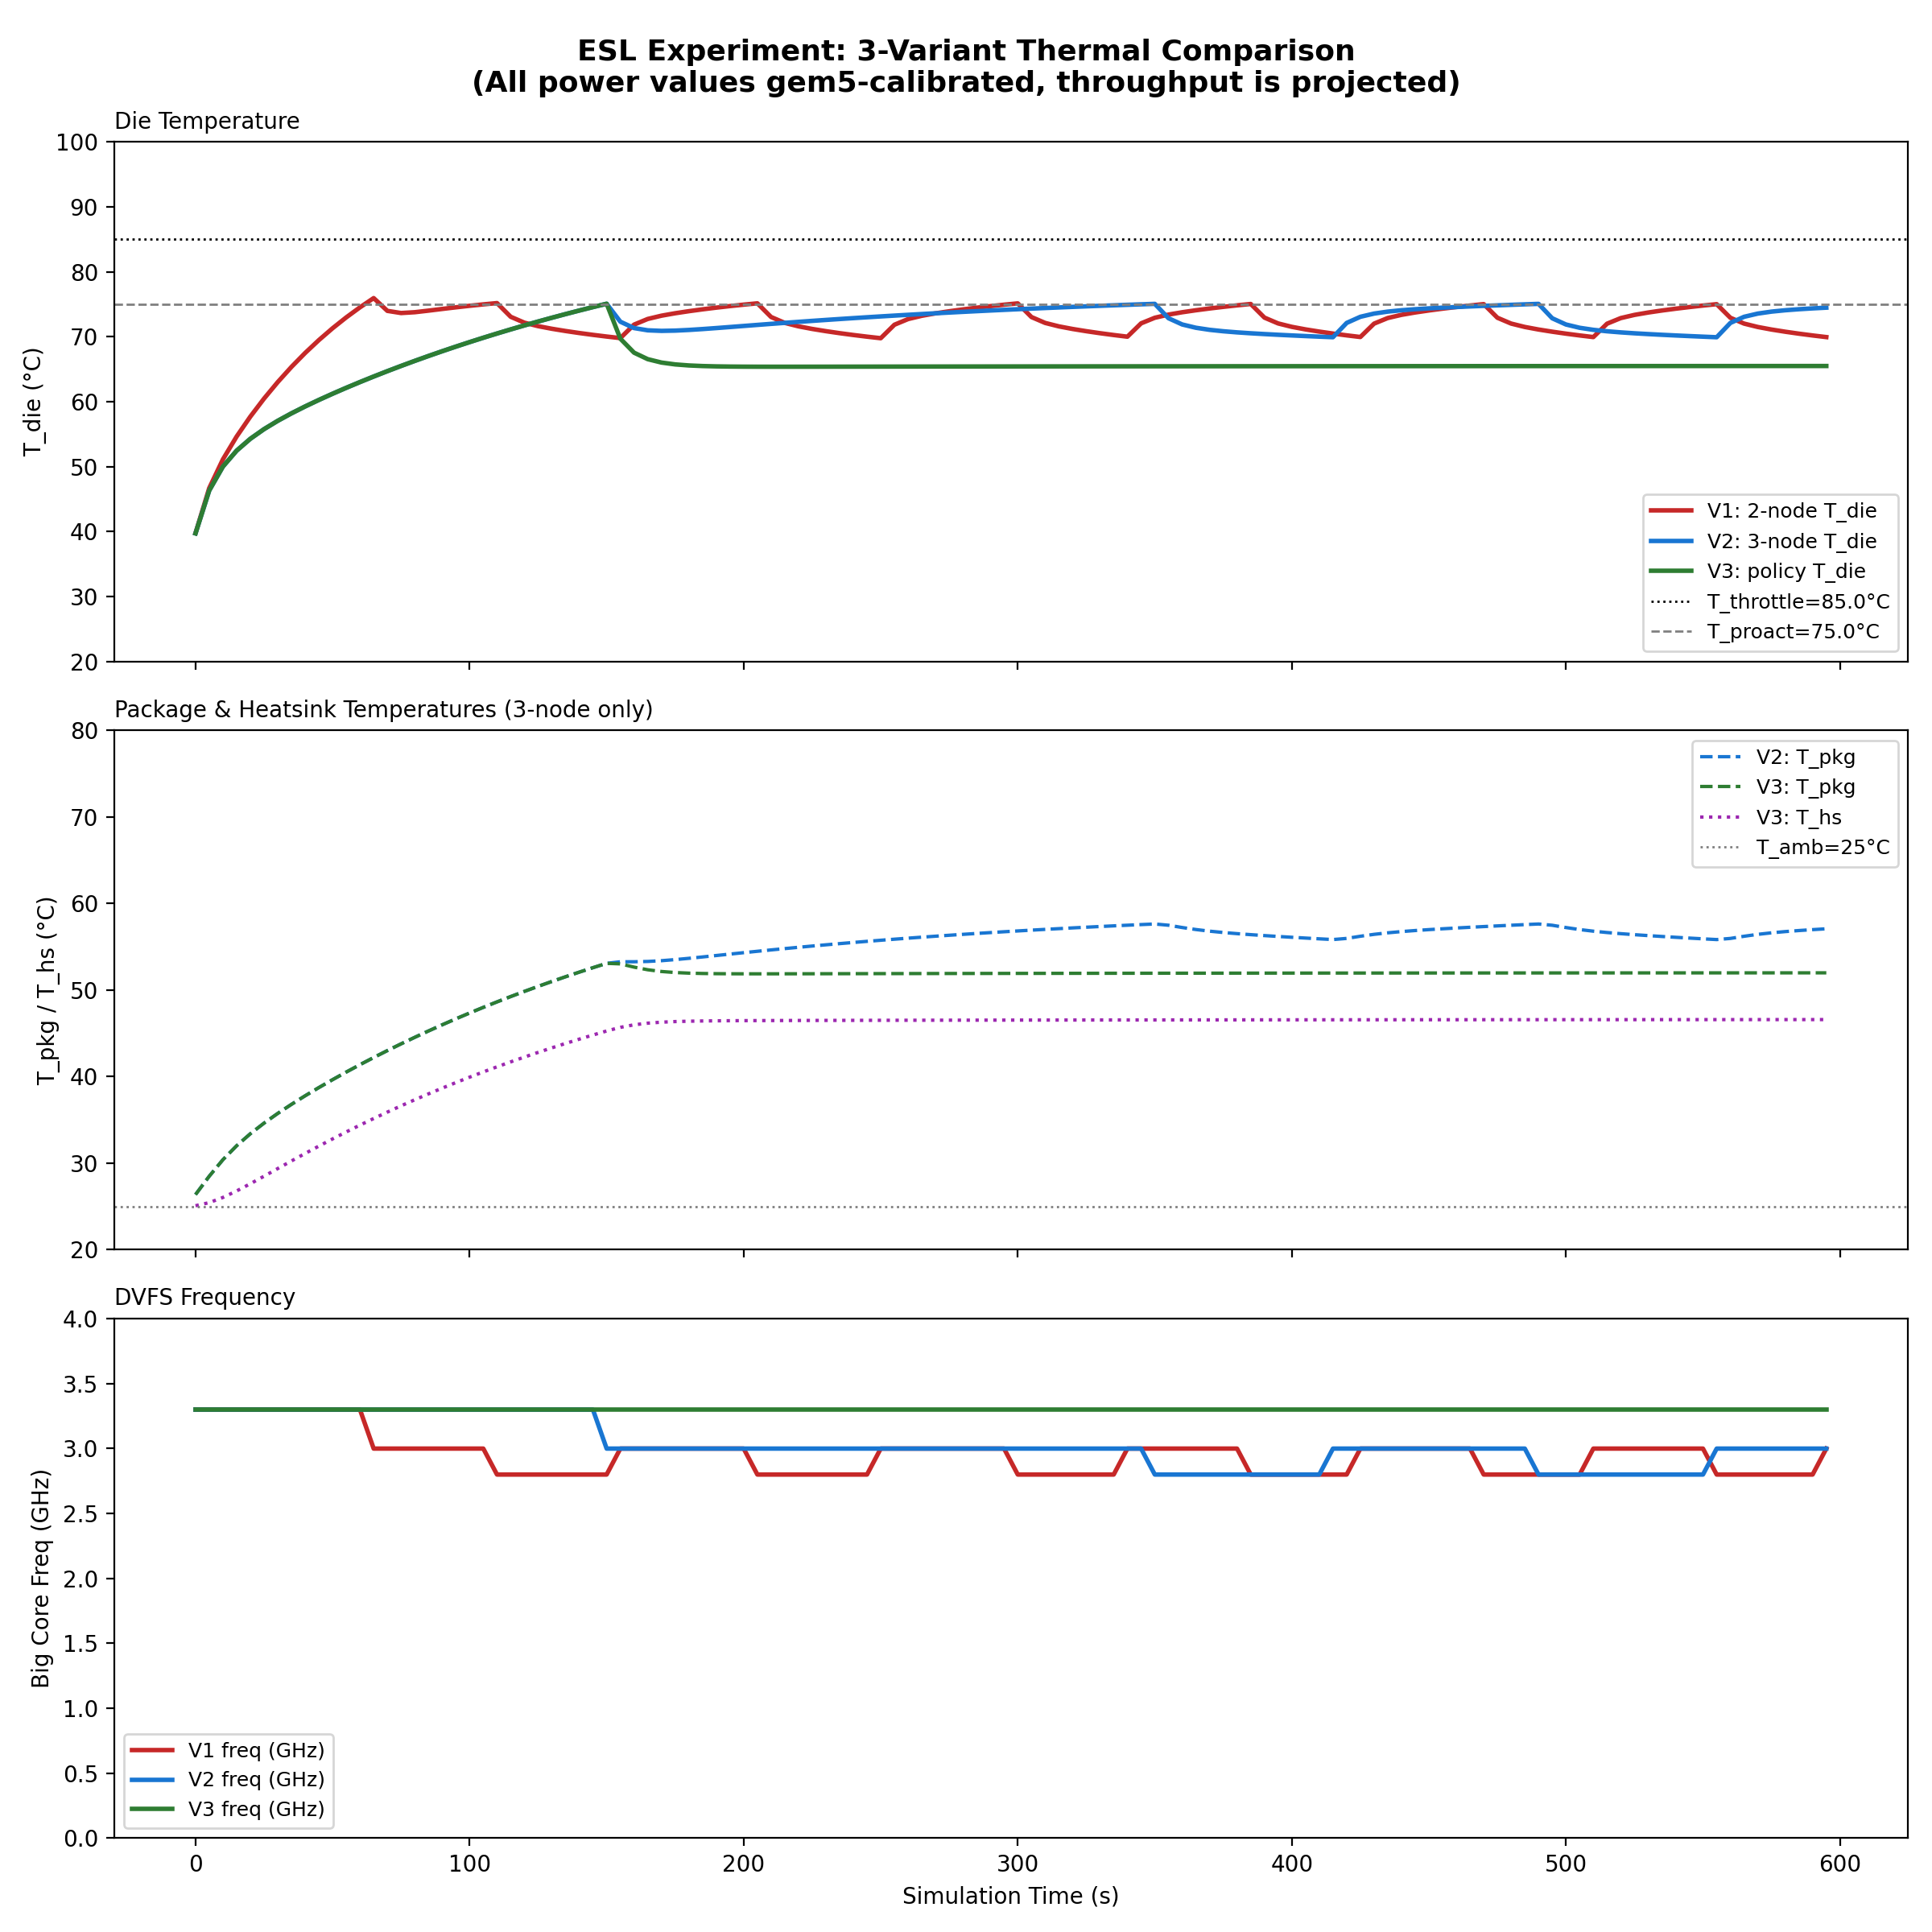
\includegraphics[width=\columnwidth]{figures/esl_fig1_thermal_comparison.png}
\caption{Transient temperature traces for all three variants under sustained peak-OPP load. Top: $T_{die}$; middle: $T_{pkg}$ and $T_{hs}$; bottom: big-cluster frequency. The 3-node model (V2, V3) defers the first intervention by 85\,s vs.\ the 2-node baseline (V1). All values are modeled.}
\label{fig:thermal_comparison}
\end{figure}

\begin{figure}[t]
\centering
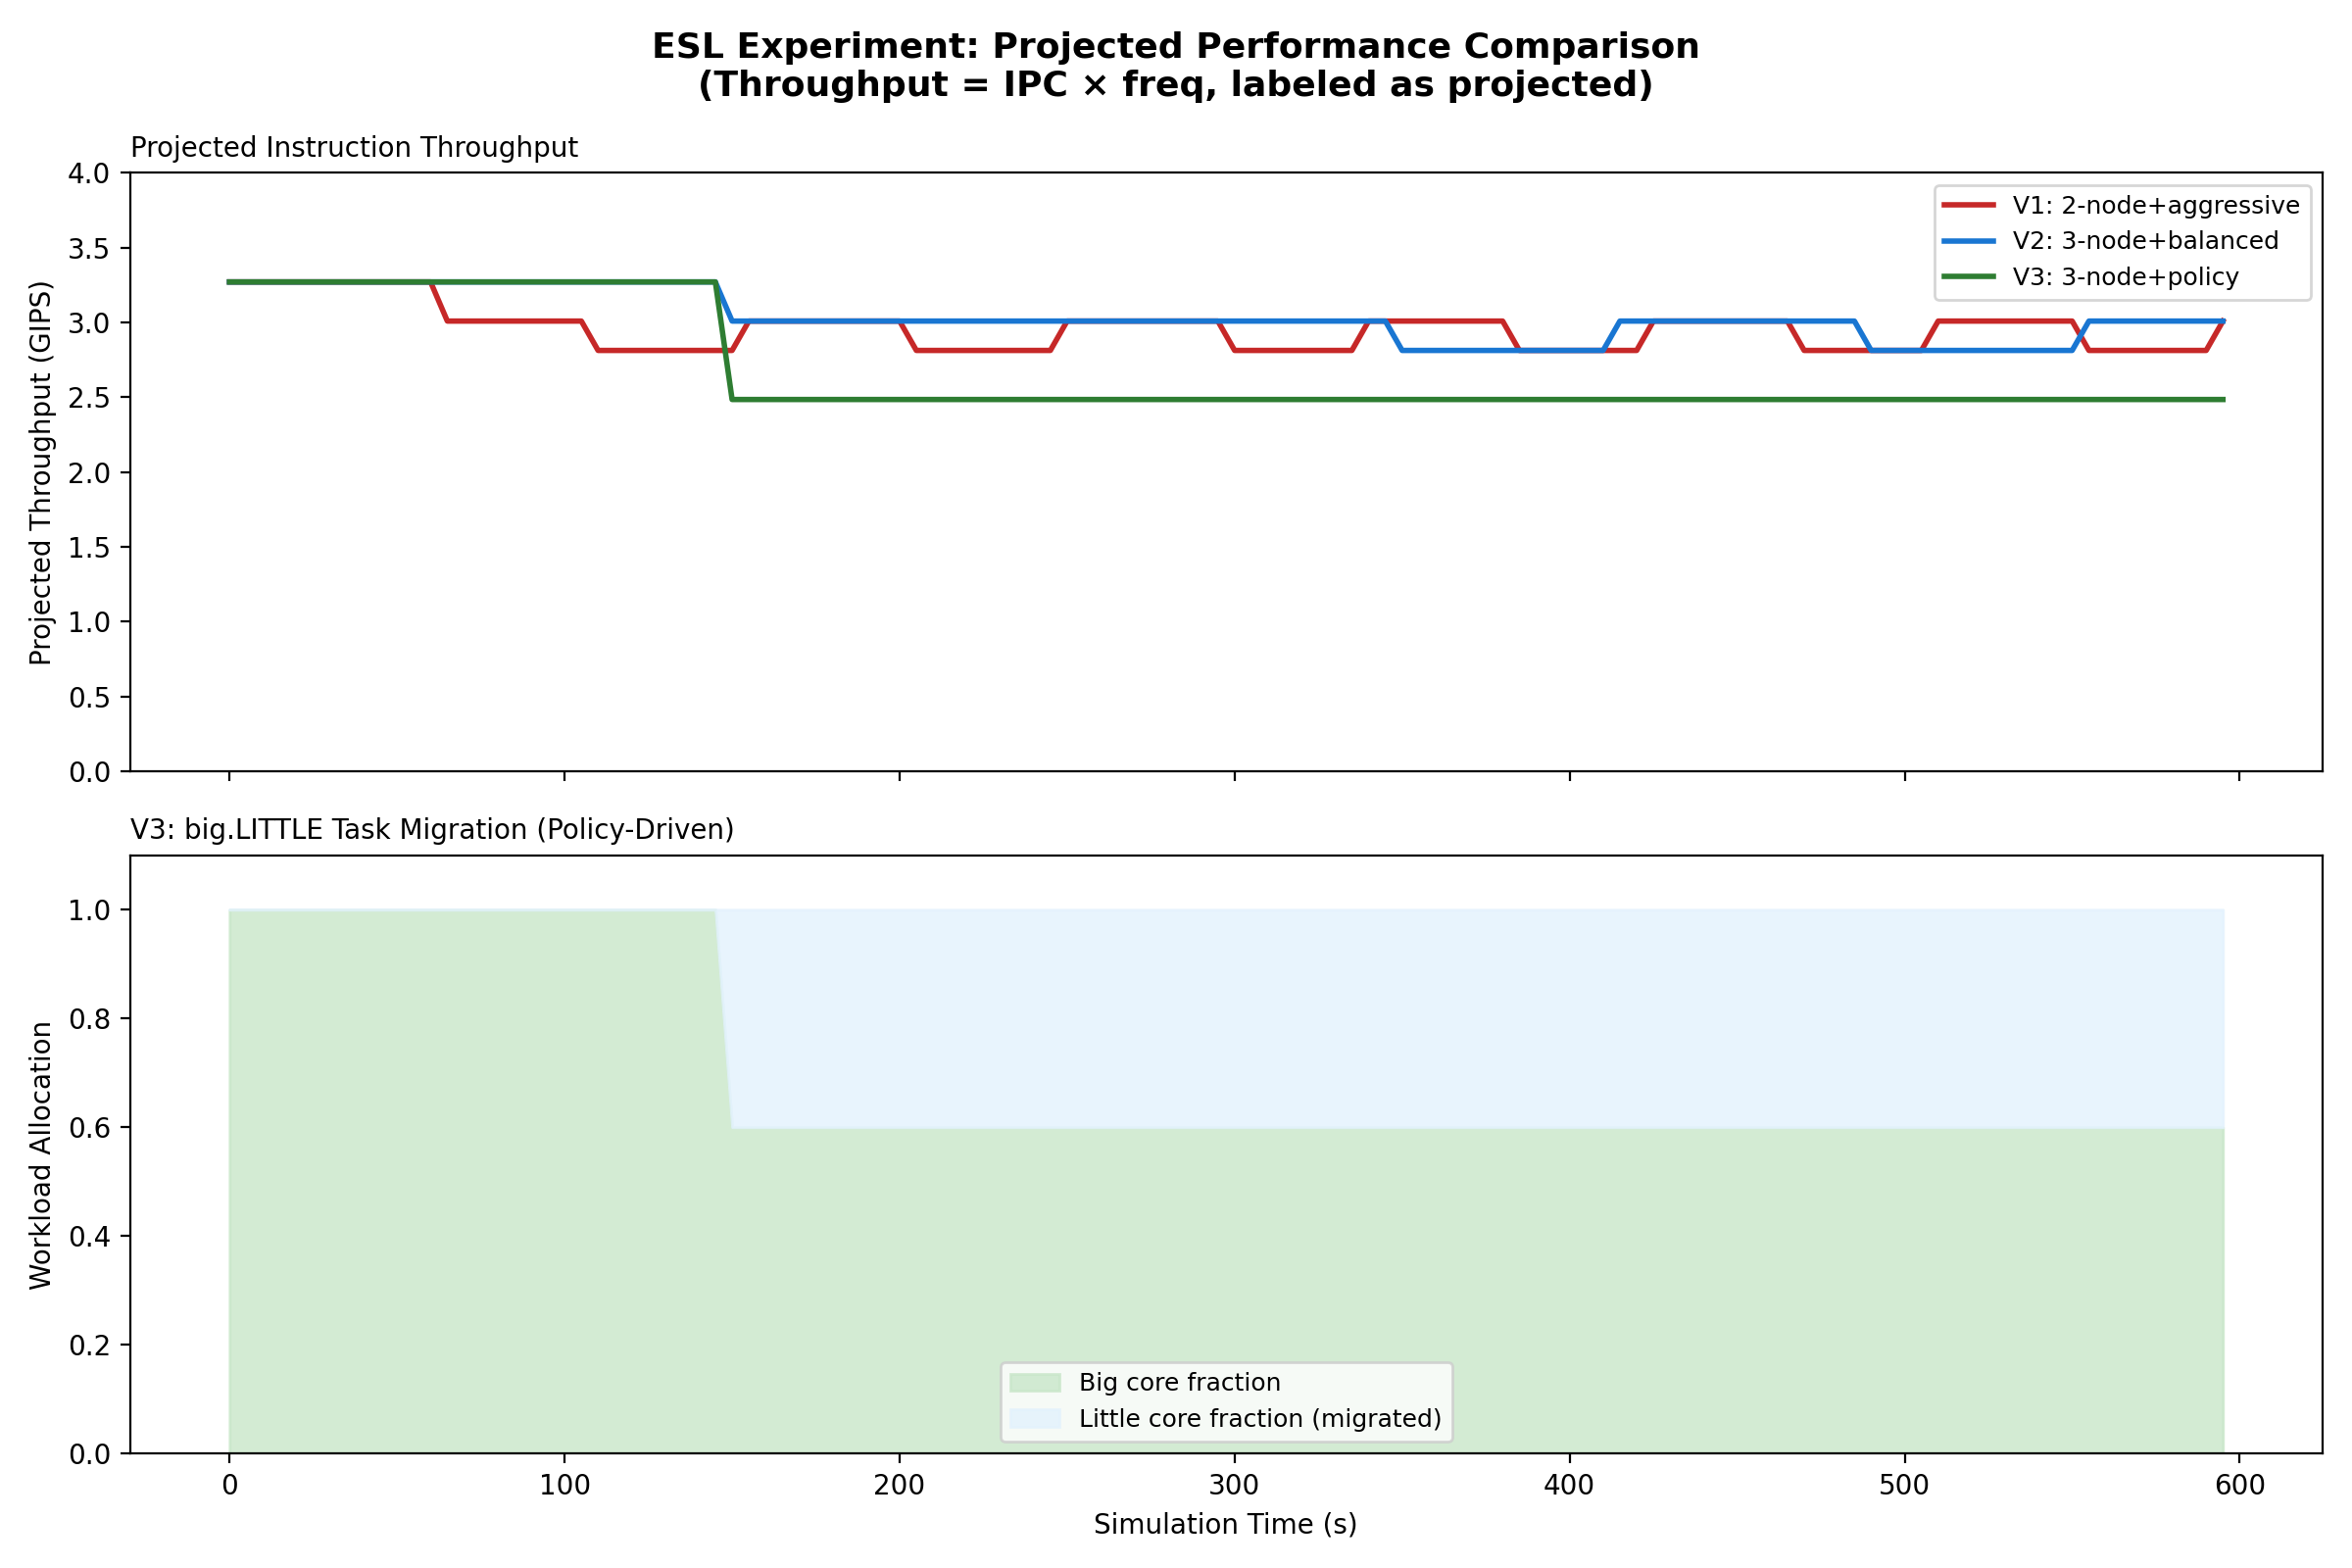
\includegraphics[width=\columnwidth]{figures/esl_fig2_performance_migration.png}
\caption{Projected throughput (GIPS) and V3 big/LITTLE workload split over 600\,s. The Phase~6 policy migrates 40\% of the workload at $t = 150$\,s, reducing DVFS events from 13 (V1) to 1, at a 12\% projected throughput cost. All values are modeled.}
\label{fig:performance_migration}
\end{figure}

\begin{table}[t]
\centering
\caption{Co-simulation summary (600\,s sustained load, all values modeled).}
\label{tab:results}
\small
\resizebox{\columnwidth}{!}{%
\begin{tabular}{lcccccc}
\hline
Variant & $T_{die}^{max}$ & $T_{pkg}^{max}$ & $T_{hs}^{max}$ & Events & First event & $\overline{\text{Perf}}$ \\
\hline
V1 2-node & 75.9°C & 57.9°C & ---    & 13        & 65\,s  & 2.96\,GIPS \\
V2 3-node & 75.1°C & 57.6°C & 50.9°C & 5         & 150\,s & 3.03\,GIPS \\
V3 policy & 75.1°C & \textbf{53.1°C} & \textbf{46.6°C} & \textbf{1} & 150\,s & 2.68\,GIPS \\
\hline
\end{tabular}%
}
\end{table}

\subsubsection{Sustained Workload}
As shown in Fig.~\ref{fig:thermal_comparison} and Table~\ref{tab:results}, the 2-node model (V1) triggers its first proactive DVFS step-down at $t = \SI{65}{\second}$, and oscillates through 13 events over the simulation. The 3-node model (V2) defers the first intervention to $t = \SI{150}{\second}$---an \textbf{85-second improvement}---because the heatsink's $\tau_{hs}=120$\,s thermal inertia absorbs the initial heat flux before $T_{die}$ reaches $T_{proact}$. V2 also sustains higher projected throughput (3.03 vs.\ 2.96\,GIPS) with 62\% fewer interventions. The similar V1/V2 peak package temperatures (57.9 vs.\ 57.6\,°C) reflect the 2-node model's lumping of package and heatsink into one node; the true 3-node observability gain is the separately-tracked $T_{hs}^{max} = 50.9\,\text{°C}$, a thermal state that V1 cannot resolve.

The Phase~6 policy (V3) replaces all DVFS oscillations with a single migration event at $t = \SI{150}{\second}$ (Fig.~\ref{fig:performance_migration}): when $T_{die} \geq 75\,\text{°C}$ and $T_{pkg} = 53\,\text{°C} \ll 65\,\text{°C}$, Tier~1 offloads 40\% of the workload to the LITTLE cluster. This lowers big-core power injection, stabilising $T_{die}$ for the remainder of the run without any frequency reduction. The package temperature ceiling drops from 57.6\,°C (V2) to \textbf{53.1\,°C} (V3). The trade-off is a 12\% reduction in projected throughput (2.68 vs.\ 3.03\,GIPS), since LITTLE-core execution is less efficient per unit power. The deferred throttling in V2 and V3 also slightly increases modeled energy consumption versus V1 (V2: +8\%), as big-cluster execution is sustained longer before any intervention.

The 24$\times$ time-constant separation ($\tau_1 = 5\,\text{s}$, $\tau_{hs} = 120\,\text{s}$) further predicts that brief bursty loads would raise $T_{die}$ without saturating $T_{pkg}$, so the 3-node model defers intervention while a 2-node model would prematurely throttle. Quantitative validation under bursty load is reserved for future work. A separate gem5 timing-mode experiment (Phase~7) observed that EAS placed a free-running workload on the LITTLE cluster (cpu1), while a pinned workload remained on cpu0, consistent with the migration mechanism modeled in V3.

\subsection{Limitations}
All results are produced by trace-driven co-simulation, not measured on physical hardware. The RC parameters are validated against gem5 configuration files and smoke-run outputs, but have not been calibrated against silicon-level thermal measurements. The migration ratio is fixed at 40\%; an adaptive controller is left as future work. Only sustained peak-OPP load is evaluated quantitatively; bursty workload analysis is limited to the analytical argument above. Finally, gem5 full-system timing-mode simulation is too slow ($\sim$250\,ms simulated per real second) to observe thermal dynamics at the $\tau_{hs} = 120$\,s time scale, which motivates the trace-driven approach used in this paper.
